\chapter{Cortical morphometry}
\setstretch{\lspac}

\section{Introduction}
\label{sec:cortex:intro}
\setstretch{\lspac}

It has been suggested that biological processes that drive horizontal (tangential) and vertical (radial) development of the cerebral cortex are separate from each other \citep{Rakic1988,Geschwind2013}, influencing cortical area and thickness independently. These two indices of cerebral morphology are uncorrelated genetically \citep{Panizzon2009, Winkler2010}, are each influenced by regionally distinct genetic factors \citep{Schmitt2008, Rimol2010_bp, Chen2012}, follow different trajectories over the lifespan \citep{OLeary2007, Hogstrom2013, Fjell2015}, and are differentially associated with cognitive abilities \citep{Schnack2015, Noble2015, Vuoksimaa2016}. Moreover, it is cortical area, not thickness, that differs substantially across species \citep{Rakic1995}. These findings give prominence to the use of surface area alongside thickness in studies of cortical morphology and its relationship to function. The literature contains a variety of approaches and terminologies for its assessment and cortical volume, which commingles thickness and area, continues to be a popular metric, thanks largely to the wide availability of voxel-based morphometry (\textsc{vbm}) \citep{Ashburner2000, Good2001, Douaud2007}. While analysing cortical thickness and cortical area separately improves specificity \citep{Rimol2012}, it may still be of interest to combine these two measurements so as to increase power to investigate non-specific challenges that could affect thickness and area simultaneously, such as auto-immune \citep{Ceccarelli2008, Zhang2016} and infectious neurological disorders \citep{Gitelman2001, Kuper2011}, or in relation to inflammatory markers \citep{Marsland2008, Zhang2015}. The contributions of this paper are threefold: we (\textsc{i}) expose certain aspects of the various methods for cortical area analysis, in particular the interpolation between surfaces at different resolutions; (\textsc{ii}) propose an improved, analytic measurement of volume; (\textsc{iii}) show that a joint analysis using the non-parametric combination \textsc{npc} \citep{Pesarin2010, Winkler2016_npc} of thickness and area provides a sensible solution to the investigation of factors that can affect cortical morphology, which can replace the analysis of cortical volume altogether.
 
\subsection{Cortical surface area}

Comparisons of area across subjects at every point in the cortex are advantageous over simple regions on interest for not depending on the definition of borders. However, they depend on registration of the cortical surface and interpolation to a common resolution. Such resampling must preserve the amount of area at local, regional and global scales, i.e., it must be mass-conservative. A well known interpolation method is the \emph{nearest-neighbour}, which can be enhanced by correction for stretches and shrinkages of the surface during the registration, as available in the function ``mris\_preproc'', part of the FreeSurfer (\textsc{fs}) software package (available at \href{http://freesurfer.net}{freesurfer.net}). Another approach is the \emph{retessellation} of the mesh of each subject to the geometry of a common grid, as proposed by \cite{Saad2004} as a way to produce meshes with similar geometry across subjects, thus allowing statistical analysis. Even though the method has been mostly used to compute areal expansion, it can be used for surface area itself, as well as for other areal quantities. A third approach is the use of the barycentric coordinates of each vertex with reference to the vertices of the common grid to \emph{redistribute} the areal quantities, in an approximately mass preserving process. Lastly, a complete framework for analysis of areal quantities was presented in \cite{Winkler2012} using a \emph{pycnophylactic} interpolation method, that is, a method that preserves areal quantities. Table~\ref{tab:overview} shows an overview of these approaches, and a detailed description is in the Methods section.

\begin{table}%[!tb]
\caption{Overview of the four different methods to interpolate surface area and areal quantities. A detailed description is in the Methods section.}
\begin{center}
\begin{small}
\begin{tabular}{@{}m{28mm}<{\raggedright}m{96mm}<{\raggedright}@{}}
\toprule
\textbf{Method} & \textbf{Description} \\ 
\midrule
Nearest-neighbour & Nearest-neighbour interpolation of areal quantities on the sphere, followed by Jacobian correction.\\
\midrule
Retessellation & Barycentric interpolation on the sphere of the native vertex coordinates.\\
\midrule
Redistributive & Vertexwise redistribution of areal quantities based on bary\-centric coordinates of the source in relation to the target.\\
\midrule
Pycnophylactic & Mass-conservative facewise interpolation method that uses the overlapping areas between faces of source and target.\\
\bottomrule
\end{tabular}
\end{small}
\end{center}
\label{tab:overview}
\end{table}

\subsection{Measuring volume and other areal quantities}

The volume of cortical grey matter is also an areal quantity, therefore requiring mass-conservative interpolation methods. Volume can be estimated through the use of voxelwise partial volume effects using volume-based representations of the brain, such as in \textsc{vbm}, or from a surface representation, in which it can be measured as the amount of tissue present between the surface placed at the site of the pia-mater, and the surface at the interface between gray and white matter. If the area of either of these surfaces is known, or if the area of a mid-surface, i.e., the surface running half-distance between pial and white surfaces \citep{vanEssen2005} is known, an estimate of the volume can be obtained by multiplying, at each vertex, area by thickness. This procedure, while providing a reasonable approximation that improves over voxel-based measurements, since it is less susceptible to various artefacts \cite[for a discussion of artefacts in \textsc{vbm}, see][]{Ashburner2009}, is still problematic as it underestimates the volume of tissue that is external to the convexity of the surface, and overestimates volume that is internal to it; both cases are undesirable, and cannot be solved by merely resorting to using an intermediate surface as the mid-surface (Fig.\ref{fig:mantle}a). Here a different approach is proposed: each face of the white surface and its matching face in the pial surface are used to define an oblique truncated pyramid, the volume of which is computed analytically, without introducing additional error other than what is intrinsic to the placement of these surfaces (Fig.\ref{fig:mantle}b for a 2-\textsc{d} schema and Fig.\ref{fig:pyramid} for 3-\textsc{d}).

\begin{figure}%[p!]
\begin{center}
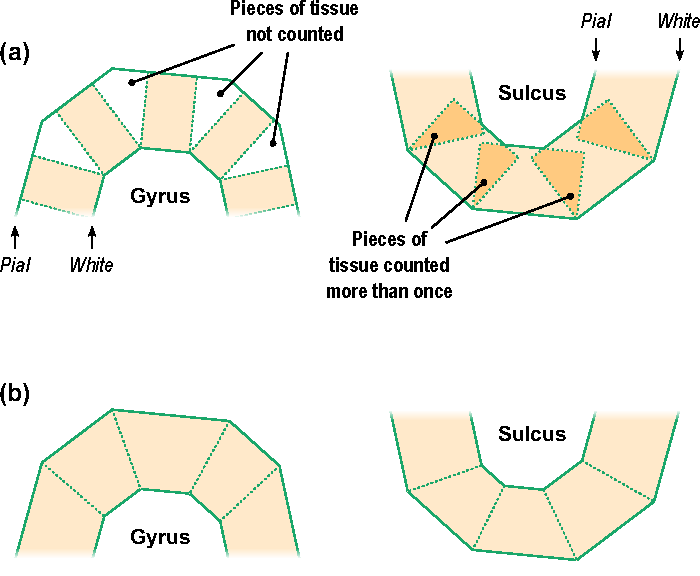
\includegraphics[width=8cm]{figures/mantle.pdf}
\caption{A diagram in two dimensions of the problem of measuring the cortical volume. (\emph{a}) If volume is computed using multiplication of thickness by area, considerable amount of tissue is left unmeasured in the gyri, or measured repeatedly in sulci. The problem is minimised, but not solved, with the use of the mid-surface. (\emph{b}) Instead, vertex coordinates can be used to compute analytically the volume of tissue between matching faces of white and pial surfaces, leaving no tissue under- or over-represented.}
\label{fig:mantle} 
\end{center}
\end{figure}

\begin{figure}%[t!]
\begin{center}
\hspace*{-.7cm}
\includegraphics[width=14.5cm]{figures/pyramid.pdf}
\caption{(\emph{a}) In the surface representation, the cortex is limited internally by the white and externally by the pial surface. (\emph{b}) and (\emph{c}) These two surfaces have matching vertices that can be used to delineate an oblique truncated triangular pyramid. (\emph{d}) The six vertices of this pyramid can be used to define three tetrahedra, the volumes of which are computed analytically.}
\label{fig:pyramid}
\end{center}
\end{figure}

Quantitative measurements, such as from positron emission tomography (\textsc{pet}), cerebral blood flow, cerebral blood volume, the mass, or number of molecules of a given compound \citep{Leahy2000, VandenHoff2005}, are all areal quantities whenever these are expressed in absolute quantities. Likewise, cerebral blood flow and volume obtained using methods based on magnetic resonance imaging (\textsc{mri}), such as arterial spin labelling (\textsc{asl}), as well as other forms of quantitative \textsc{mri}, as those involving contrast enhancement \citep{Parker2003}, quantitative magnetisation transfer \citep{Levesque2010, Harrison2015}, or quantitative assessment of myelination, are also areal quantities that require mass conservation when measured in absolute terms. The methods used for statistical analysis surface area can be applied for these areal quantities as well.

\subsection{Non-parametric combination (\textsc{npc})}

Instead of volume, a joint approach can be considered for the analysis of thickness and area. Classical multivariate tests such as \textsc{mancova}, however, do not inform the direction of effects, and are based on assumptions that are known not to hold for surface area, such as normality. Rather, the permutation-based non-parametric combination (\textsc{npc}) \citep{Pesarin2010, Winkler2016_npc} provides a test for directional as well as two-tailed hypotheses, and is based on minimal assumptions, mainly that of exchangeability, that is, swapping one datum for another keeps the data just as likely.

The \textsc{npc} consists of, in a first phase, testing separately hypotheses on each available metric using permutations that are performed in synchrony; these tests are termed \emph{partial tests}. The resulting statistics for each and every permutation are recorded, allowing an estimate of the complete empirical cumulative distribution function (cdf) to be constructed for each one. In a second phase, the empirical p-values for each test are combined, for each permutation, into a \emph{joint statistic}. As the joint statistic is produced from the previous permutations, an estimate of its empirical cdf function is immediately known, and so is its corresponding p-value.

As originally proposed and as described above, \textsc{npc} is not practicable in brain imaging: as the statistics for all partial tests for all permutations need to be recorded, an enormous amount of space for data storage is necessary. However, even if storage space were not a problem, the discreteness of the p-values for the partial tests is problematic when correcting for multiple testing, because with thousands of vertices in a surface, ties occur frequently, further causing ties among the combined statistics. If too many tests across an image share the same most extreme statistic, correction for the multiplicity, while still valid, is less powerful \citep{Westfall1993, Pantazis2005}. The most obvious workaround --- run an ever larger number of permutations to break the ties --- may not be possible for small sample sizes, or when possible, requires correspondingly larger data storage. The solution to this problem is loosely based on the direct combination of the test statistics, by converting the statistics of the partial tests to values that behave as p-values using the asymptotic distribution of the statistics, and using these for the combination \citep{Winkler2016_npc}.

\paragraph{Combining functions}

The null hypothesis of the \textsc{npc} is that the null hypotheses for all partial tests are true, and the alternative is that any test is false, which is the same that a union-intersection test (\textsc{uit}) \citep{Roy1953}. The rejection region depends on how the combined statistic is produced. Various combining functions can be considered, particularly those used in meta-analyses, such as Fisher's combination of p-values, i.e., $T=-2\sum_k\ln(p_k)$ \citep{Fisher1932} and Stouffer's combination of $z$-statistics, i.e., $T = \sum_k \Phi^{-1}(1-p_k)/\sqrt{K}$ \citep{Stouffer1949}, where $T$ is the test statistic for the joint test, $p_k$ is the p-value of the $k$-th out of $K$ partial tests, and $\Phi^{-1}$ is the probit function. These and most other combining functions, related statistics and their distributions were originally derived under the assumption of independence among the partial tests, which is not always valid, particularly under the tenable hypothesis of shared environmental effects affecting both area and thickness. Such lack of independence is not a problem for \textsc{npc}: the synchronised permutations implicitly capture the dependencies among the tests that would cause a parametric combination to be invalid, even if using the same combining functions.

\section{Method}
\label{sec:cortex:method}

The general workflow for surface-based morphometry consists of the generation of a surface-representation of the cortex and its subsequent homeomorphic transformation into a sphere. Vertices of this sphere are shifted tangentially along its surface to allow alignment matching a particular feature of interest of a reference brain (i.e., an atlas), such as sulcal depth, myelin content, or functional markers. Once registration has been done, interpolation to a common grid is performed; it is at the resolution of this grid that analyses across subjects are performed. While the order of these processing stages remains generally fixed, the stage in which areal quantities are calculated or obtained varies according to the method: for the nearest neighbour, redistributive, and pycnophylactic methods, these are computed in the native space, using native geometry. With the retessellation method, area is computed in native space, with a new geometry produced after interpolation of the surface coordinates to the common grid. An overview of the whole process is in Figure~\ref{fig:flowchart}.

\begin{figure}[p!]
\begin{center}
\hspace*{-.2cm}
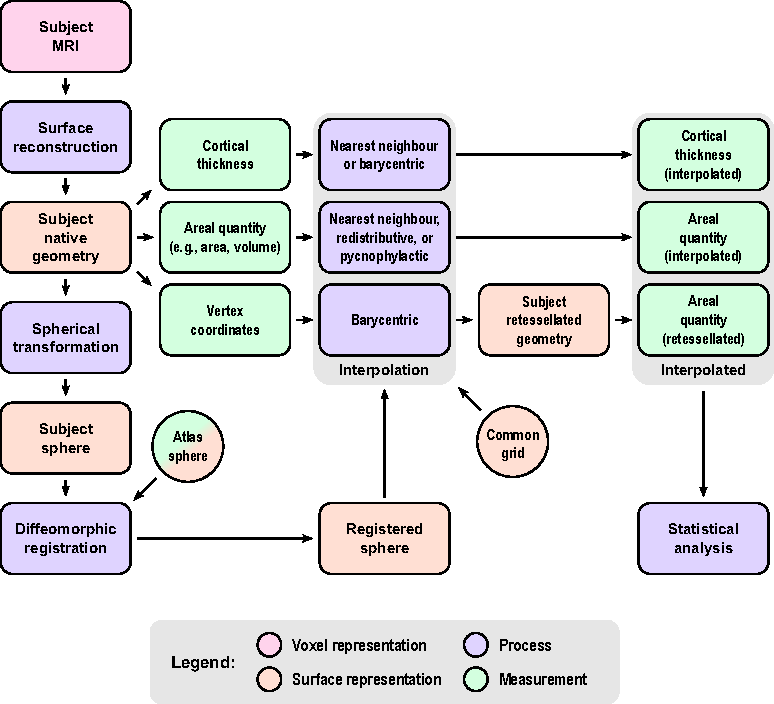
\includegraphics{figures/flowchart.pdf}
\caption{An overview of the steps for the analysis of surface area using different methods. The subject magnetic resonance images are used to reconstruct a pair of surfaces (pial and white) representing the cortex, which initially are in the subject space and individual geometry. From this pair of surfaces, cortical thickness can be measured. From the same surfaces, area and volume can be measured. Finally, the coordinates of the vertices can be stored for subsequent use. The subject native surfaces are homeomorphically transformed to a sphere, registered to a spherical atlas, and used for the interpolation, which for thickness can be either nearest neighbour or barycentric, for area can be nearest neighbour, redistributive or pycnophylactic, and for the vertex coordinates can be barycentric. In the latter, the interpolation of coordinates allows the construction of a new retessellated surface in subject space, from which area can alternatively be measured. The interpolated quantities are then ready to undergo statistical analyses. See references in the main text.}
\label{fig:flowchart}
\end{center}
\end{figure}

We evaluate (1) if and where the four different interpolation methods (nearest neighbour, retessellation, redistributive and pycnophylactic) differ; (2) if and where these methods vary according to the resolution of the common grid used as target; (3) if and where the two ways of measuring volumes (the product method and the analytic method) differ from each other; (4) how the \textsc{npc} results would relate to the separate analyses of thickness, area and volume.

\subsection{Subjects}

In the period 1986--88, 121 preterm newborns with very low birth weight (\textsc{vlbw}; $\leqslant$~1500g) were admitted to the Neonatal Intensive Care Unit at the St.\ Olav University Hospital in Trondheim, Norway. At age 20, a total of 41 \textsc{vlbw} subjects consented to participate and had usable \textsc{mri} data. The term-born controls were born at the same hospital in the same period. A random sample of women with parities 1 or 2 was selected for follow-up during pregnancy. At birth, 122 children with birth weight above the tenth percentile for gestational age from this sample were included as controls. At age 20, a total of 59 control subjects consented to participate and had usable \textsc{mri} data. Further details can be found in \citet{Martinussen2005, Skranes2007}.

\subsection{Data acquisition}

\textsc{mri} scanning was performed on a 1.5~T Siemens \textsc{magnetom} Symphony scanner equipped with a quadrature head coil. In each scanning session, two sagittal $T_1$-weighted magnetization prepared rapid gradient echo (\textsc{mprage}) scans/sequences were acquired (echo time = 3.45~ms, repetition time = 2730~ms, inversion time = 1000~ms, flip angle = 7\degree; field of view = 256~mm, voxel size = 1 $\times$ 1 $\times$ 1.33~mm, acquisition matrix 256 $\times$ 192 $\times$ 128).  

\subsection{Reconstruction of the cortical surface}

We used the method implemented in the FreeSurfer software package \cite[version 5.3.0;][]{Dale1999,Fischl1999_cortical}: $T_1$-weighted images are first corrected for magnetic field inhomogeneities and then skull-stripped \citep{Segonne2004}. Voxels belonging to the white matter (\textsc{wm}) are identified based on their locations, on their intensities, and on the intensities of the neighbouring voxels. A mass of connected \textsc{wm} voxels is produced for each hemisphere, using a six-neighbours connectivity scheme, and a mesh of triangular faces is tightly built around this mass, using two triangles for each externally facing voxel side. The mesh is smoothed taking into account the local intensity in the original images \citep{Dale1993}, at a subvoxel resolution. Defects are corrected \citep{Fischl2001,Segonne2007} to ensure that the surface has the same topological properties of a sphere. A second iteration of smoothing is applied, resulting in a realistic representation of the interface between gray and white matter (the \emph{white surface}). The external cortical surface (the \emph{pial surface}), which corresponds to the pia mater, is produced by nudging outwards the white surface towards a point where the tissue contrast is maximal, between gray matter and \textsc{csf}, maintaining constraints on its smoothness while preventing self-intersection. Cortical thickness is measured as the distance between the matching vertices of these two surfaces \citep{Fischl2000}.

\subsection{Measurement of areal quantities}

Areal quantities are measured in native space, i.e., before spherical transformation and registration. For the retessellation method, the measurement is made in native space after the surface has been reconstructed to a particular resolution; for nearest neighbour, redistributive, and pycnophylactic, measurement uses native space, with the original, subject-specific mesh geometry. 

\paragraph{Cortical area}

For a triangular face $ABC$ of the surface representation, with vertex coordinates $\mathbf{a}=[x_A \; y_A \; z_A]'$, $\mathbf{b}=[x_B \; y_B \; z_B]'$, and $\mathbf{c}=[x_C \; y_C \; z_C]'$, the area is $|\mathbf{u} \times \mathbf{v}|/2$, where $\mathbf{u} = \mathbf{a}-\mathbf{c}$, $\mathbf{v} = \mathbf{b}-\mathbf{c}$, $\times$ represents the cross product, and the bars $|\;|$ represent the vector norm. Although the area per face (i.e., the \emph{facewise} area) can be used in subsequent steps, it remains the case that most software packages can only deal with values assigned to each vertex of the mesh (i.e., \emph{vertexwise}). Conversion from facewise to vertexwise is achieved by assigning to each vertex one-third of the sum of the areas of all faces that have that vertex in common \citep{Winkler2012}.

\paragraph{Cortical volume}

The conventional method for computing surface-based volume consists of computing the area at each vertex as above, then multiplying this value by the thickness at that vertex, in a procedure that leaves tissue under- or over-represented in gyri and sulci (Fig.\ref{fig:mantle}). Instead, volumes can be computed using the three vertices that define a face in the white surface and the three matching vertices in the pial surface, defining an \emph{oblique truncated triangular pyramid}, which in turn is perfectly subdivided into three tetrahedra. The volumes of these are computed analytically, summed, and assigned to each face of the surface representation, viz.:

\begin{itemize}[leftmargin=*]
\item[1.] For a given face $A_w B_w C_w$ in the white surface, and its corresponding face $A_p B_p C_p$ in the pial surface, define an oblique truncated triangular pyramid.
\item[2.] Split this truncated pyramid into three tetrahedra, defined as:
$$
\begin{array}{lcllllll}
T_1 &=& (&A_w,&B_w,&C_w,&A_p&)\\
T_2 &=& (&A_p,&B_p,&C_p,&B_w&)\\
T_3 &=& (&A_p,&C_p,&C_w,&B_w&)
\end{array}$$
This division leaves no volume under- or over-represented.
\item[3.] For each such tetrahedra, let $\mathbf{a}$, $\mathbf{b}$, $\mathbf{c}$ and $\mathbf{d}$ represent its four vertices in terms of coordinates $[x\;y\;z]'$. Compute the volume as $|\mathbf{u}\cdot(\mathbf{v} \times \mathbf{w})|/6$, where $\mathbf{u} = \mathbf{a}-\mathbf{d}$, $\mathbf{v} = \mathbf{b}-\mathbf{d}$, $\mathbf{w} = \mathbf{c}-\mathbf{d}$, the symbol $\times$ represents the cross product, $\cdot$ represents the dot product, and the bars $|\;|$ represent the vector norm.
\end{itemize}

\noindent
Computation can be accelerated by setting $\mathbf{d}=A_p$, the common vertex for the three tetrahedra, such that the vector subtractions can happen only once. Conversion from facewise volume to vertexwise is possible, and done in the same manner as for facewise area. The above method will be the default in the next FreeSurfer release.

\subsection{Spherical transformation}

The white surface is homeomorphically transformed to a sphere \citep{Fischl1999_intersubject}, thus keeping a one-to-one mapping between faces and vertices of the native geometry (white and pial) and the sphere. All these surfaces comprise triangular faces exclusively. Measurements of interest obtained from native geometry or in native space, such as area and thickness, are stored separately and are not affected by the transformation, nor by registration (next step; see diagram in \emph{SI~§1}).

\subsection{Registration}

Various strategies are available to put all surfaces in register and allow comparisons between, including the one used by FreeSurfer \citep{Fischl1999_intersubject}, Spherical Demons (\textsc{sd}) \citep{Yeo2010}, Multimodal Surface Matching (\textsc{msm}) \citep{Robinson2014}, among others. From these, methods that are diffeomorphic (i.e., smooth and invertible) should be favoured. Methods that are not diffeomorphic by construction, but that in practice produce invertible and smooth warps can, in principle, be used for registration for areal analyses. For these analyses, the FreeSurfer method was used; a side comparison with \textsc{sd} is in the Supplementary Information).

\subsection{Interpolation methods}

Statistical comparisons require meshes with a common resolution where each point (vertex, face) represents homologous regions across individuals. A mesh that can act as a common grid is a geodesic sphere constructed by iterative subdivision of the faces of a regular (Platonic) icosahedron. A geodesic sphere has many advantages as the target for interpolation: ease of computation, edges of roughly similar sizes and, if the resolution is fine enough, edge lengths that are much smaller than the diameter of the sphere \citep{Kenner1976}. We compared four different interpolation methods each at three different mesh resolutions: \textsc{ic}3 (lowest resolution, with 642 vertices and 1280 faces), \textsc{ic}5 (intermediate resolution, with 10242 vertices and 20480 faces),  and \textsc{ic}7 (163842 vertices and 327680 faces).

\paragraph{Nearest neighbour interpolation}

The well known nearest neighbour interpolation does not guarantee preservation of areal quantities, although modifications can be introduced to render it approximately mass conservative: for each vertex in the target, the closest vertex is found in the source sphere, and the area from the source vertex is assigned to the target vertex; if a given source vertex maps to multiple target vertices, its area is divided between them so as to preserve the total area. If there are any source vertices that have not been represented in the target, for each one of these, the closest target vertex is located, and the corresponding area from the source surface is incremented to any area already stored on it. This method ensures that the total area after mapping into the group surface remains unchanged. This process is a surface equivalent of Jacobian correction\footnote{Not to be confused with the computation of the Jacobian itself, that is defined, for the $i$-th vertex, as $J_i = \frac{A^S_i}{A^w_i}\frac{\sum_i A^w_i}{\sum_i A^S_i}$, where $A^S_i$ is the area of the vertex in the source (registered) sphere, $A^w_i$ is the area of the same vertex in the white surface (native space and native geometry), and the sums are over the entire surface, i.e., all vertices.} used in volume-based methods in that it accounts for stretches and shrinkages while preserving the overall amount of areal quantities. The nearest neighbour is currently the default method in FreeSurfer.

\paragraph{Retessellation of the native geometry}

This method appeared in \citet{Saad2004}. It consists of generating a new mesh by interpolating not the area assigned to vertices, but the coordinates of the corresponding vertices in the native geometry. The set of three coordinates is used, together with the connectivity scheme between vertices from the common grid, to construct a new mesh that has overall similar shape as the original brain, but with the geometry of the common grid. The areas for each face (or vertex) can be computed from this new mesh, and therefore be used for statistical comparisons among subjects. Equivalently, the coordinates of each vertex can be treated as a single vector, and the barycentric interpolation can be performed in a single step as:

$$
\left[
\begin{array}{c}
x_{P} \\
y_{P} \\
z_{P}
\end{array} \right] = \left[
\begin{array}{ccc}
x_{A} & x_{B} & x_{C} \\
y_{A} & y_{B} & y_{C} \\
z_{A} & z_{B} & z_{C} \\
\end{array}
\right] \left[
\begin{array}{c}
\delta_{A} \\
\delta_{B} \\
\delta_{C}
\end{array} \right]
$$

\noindent
where $x,y,z$ represent the coordinates of the triangular face $ABC$ and of the interpolated point $P$, both in native geometry, and $\delta$ are the barycentric coordinates of $P$ with respect to the same face after the spherical transformation. From the four methods considered in this paper, this is the only one that does not directly interpolate either area or areal quantities, but the mesh in native space.

\paragraph{Redistribution of areas}

This method works by splitting the areal quantity present in each vertex from the source sphere using the proportion given by the barycentric coordinates of that vertex in relation to the face in the target sphere (common grid) on which it lies, redistributing these quantities to the three vertices that constitute that face in the target. If some quantity was already present in these target vertex (e.g., from other source vertices lying on the same target face), that is incremented. The method is represented by:

$$
Q^T_i = \sum_{f=1}^F\sum_{v=1}^{V_f} Q^S_{vf}\delta_{ivf}
$$

\noindent
where $Q^S_{vf}$ is the areal quantity in the source vertex $v$, $v\in\left\{1, \ldots, V_f \right\}$ lying on the target face $f$, $f\in\{1,\ldots,F\}$, $F$ being the number of faces that meet at the target vertex $i$, and $\delta_{ivf}$ is the barycentric coordinate of $v$, lying on face $f$, and in relation to the target vertex $i$. This method has similarities with the conventional barycentric interpolation (as used for the interpolation of coordinates in the retesselation method). The key difference is that in the barycentric interpolation, it is the barycentric coordinates of the target vertex in relation to their containing source face that are used to weight the quantities, in a process that therefore is not mass conservative. Here it is the barycentric coordinates of the source vertex in relation to their containing target face that are used; the quantities are split proportionately, and redistributed across target vertices.

\paragraph{Pycnophylactic interpolation}

The ideal interpolation method should conserve the areal quantities globally, regionally and locally. In other words, the method has to be \emph{pycnophylactic}. This is accomplished in this method by assigning, to each face in the target sphere, the areal quantity of all overlapping faces from the source sphere, weighted by the fraction of overlap between them \citep{Markoff1973, Winkler2012}. It operates on the faces directly, not on vertices. The area (or any other areal quantity) is transferred from source to target surface via weighting by the overlapping area between any pairs of faces. The interpolated areal quantity, $Q^{T}_{i}$, of a face $i$ in the target surface, that overlaps with $F$ faces from the source surface, is given by:

$$
Q^{T}_{i} = \sum_{f=1}^{F} \frac{A^{O}_{f}}{A^{S}_{f}} Q^{S}_{f}
$$

\noindent
where $A^{S}_{f}$ is the area of the $f$-th overlapping face from the source sphere, which contains a quantity $Q^{S}_{f}$ of some areal measurement (such as the surface area measured in the native space), and $A^{O}_{f}$ is the overlapping area with the face $i$.

\paragraph{Correction for unequal face sizes and smoothing}

Regardless of the interpolation method, larger faces in the common grid inherit larger amounts of areal quantities. If the analysis will compare regions that are topographically distinct, or if the data are to be smoothed, a correction for different face sizes is needed \citep{Winkler2012}. For facewise data, it consists of weighting the the areal quantity at each face or vertex, after interpolation, by a constant that depends on the respective area in the common grid. Smoothing was considered at two levels for the comparison of areal interpolation and volume methods: no smoothing, and smoothing with a Gaussian kernel with full width at half maximum (\textsc{fwhm}) of 10~mm, small so as to preserve the effect of different resolutions being investigated. For the comparison between \textsc{vlbw} and controls, 30~mm, as in \citet{Skranes2013}.

\subsection{Statistical analysis}

The statistical analysis was performed using \textsc{palm} -- Permutation Analysis of Linear Models (available at \href{http://fsl.fmrib.ox.ac.uk}{fsl.fmrib.ox.ac.uk}) \citep{Winkler2014, Winkler2016_npc}. The number of permutations was set at 1000, followed by approximation of the tail of the distribution by a generalised Pareto distribution (\textsc{gpd}) \citep{Winkler2016_fast}, and familywise error rate correction (\textsc{fwer}) was applied considering both hemispheres and both test directions for the null hypothesis of no difference between both subject groups. Analyses were performed separately for cortical thickness, area, and volume (both methods), and also using \textsc{npc} for the joint analysis of thickness and area (Figure~\ref{fig:flowstats}.

\begin{figure}[tp!]
\begin{center}
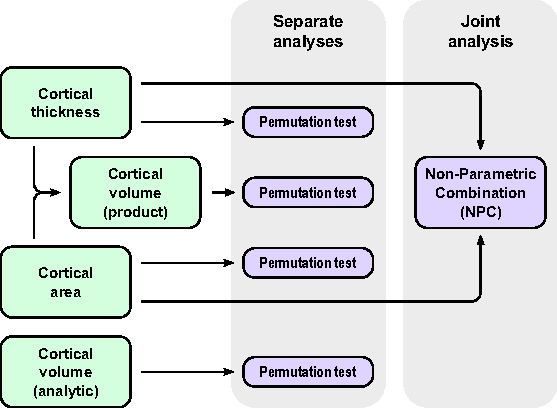
\includegraphics{figures/flowstats.pdf}
\caption{Overview of the separate and joint analyses of thickness, area and volume.}
\label{fig:flowstats}
\end{center}
\end{figure}

\subsection{Presentation of results}

The large number of scenarios evaluated, that involved two different registration and four different interpolation methods, three grid resolutions, two different smoothing levels, four different indices of cortical morphology, plus \textsc{npc}, resulted in more than 16 thousand maps and Bland-Altman plots \citep{Bland1986}. These have been organised in a set of browsable pages accessible at \href{http://bit.ly/2cHJFQC}{http://bit.ly/2cHJFQC}. These constitute the Supplementary Information, and their inspection is encouraged. The SI also includes high resolution and complementary views of the figures shown in the main text.

\section{Results}
\label{sec:cortex:results}

\subsection{Preservation of areal quantities}

At the highest resolution of the common grid used as the interpolation target (\textsc{ic}7), all methods preserve generally well the global amount of surface area, and therefore, of other areal quantities. At lower resolutions, massive amounts of area are lost with the retessellation method: about 40\% on average for \textsc{ic}3 and 9\% for \textsc{ic}5, although only 1\% for \textsc{ic}7. Areal losses, when existing, tend to be uniformly distributed across the cortex (Fig.\ref{fig:diff+corr}, upper panels), with no trends affecting particular regions and, except for retessellation, can be substantially alleviated by smoothing (\emph{SI~§2}).

\begin{figure}[p!]
\begin{adjustbox}{addcode={\begin{minipage}{\width}}{
\caption{Pairwise average differences (in mm$^2$) and correlations between the four interpolation methods, using the \textsc{ic}7 as target, with or without smoothing with a Gaussian kernel of \textsc{fwhm} = 10~mm, projected to the average white surface. Although the four methods differ, with some leading to substantial, undesirable losses and gains in surface area, and the introduction of noise manifested by lower correlations, the average variation was zero for nearest neighbour, redistributive and pycnophylactic. The retessellation method led to substantial losses of area that could not be recovered or compensated by blurring. Although this method showed excellent correlation with pycnophylactic, quantitative results after interpolation are biased downwards. For the medial views, for the right hemisphere, for \textsc{ic}3 and \textsc{ic5}, and for projections to the pial and inflated surfaces, consult the Supplemental Material.}
\label{fig:diff+corr}
\end{minipage}},rotate=90,center}
\includegraphics[scale=1.1]{figures/diff+corr.pdf}
\end{adjustbox}
\end{figure}

\subsection{Differences between interpolation methods}

While there are no spatial trends in terms of areal gains or losses, the inexactness of some interpolation methods introduces noise that substantially reduces their correlation when assessed between subjects (Fig.\ref{fig:diff+corr}, lower panels). The only exception is between the retessellation and the pycnophylactic methods, which have near perfect correlation even without any smoothing. Smoothing increases the correlation between all methods to near unity throughout the cortex (\emph{SI~§2a}). At the subject level, the spatial correlation between the nearest neighbour and the pycnophylactic methods is only about 0.60, although approaching unity when the subjects are averaged (\emph{SI~§2b}). Smoothing leads to a dramatic improvement on agreement, causing nearest neighbour to be nearly indistinguishable from the pycnophylactic method. The redistributive method performed in a similar manner, although with a higher correlation without smoothing, about 0.75 (\emph{SI~§2b}).

\subsection{Cortical volume measurements}

At the local scale, differences between the product and the analytic methods to estimate volume is as high as 20\% in some regions (\emph{SI~§3}), an amount that could not be alleviated by smoothing or by changes in resolution. As predicted by Fig.\ref{fig:mantle}, differences were larger in the crowns of gyri and depths of sulci, in either case with the reverse polarity (Fig.\ref{fig:maps_vols}, upper panels). The vertexwise correlation between the methods across subjects, however, was in general very high, approaching unity throughout the whole cortex, with or without smoothing, and at different resolutions. In regions of higher sulcal variability, however, the correlations were not as high, sometimes as low as 0.80, such as in the insular cortex and at the confluence of parieto-occipital and calcarine sulci, between the lingual and the isthmus of the cingulate gyrus (Fig.\ref{fig:maps_vols}, lower panels). At least in the case of the insula, this effect may be partly attributed to a misplacement of the white surface in the region lateral to the claustrum \citep{Glasser2016}.

\begin{figure}[t!]
\begin{center}
\includegraphics[scale=1.1]{figures/vols_diff+corr.pdf}
\end{center}
\caption{Average difference (in mm$^3$) between the two methods of assessing volume and their correlation (across subjects), using the highest resolution (\textsc{ic}7) as the interpolation target, projected to the average inflated surface. As predicated from Fig.~\ref{fig:mantle}, differences are larger in the crowns of gyri and in the depths of sulci, with gains/losses in volume in these locations following opposite patterns. Although the correlations tend to be generally high, and increase with smoothing, they are lower in regions of higher inter-individual morphological variability, such as at the anterior end of the cuneus, and in the insular cortex. For \textsc{ic}3 and \textsc{ic5}, and for projections to the white and pial surfaces, consult the Supplemental Material.}
\label{fig:maps_vols}
\end{figure}

\subsection{Variability of thickness, area and volume}

Regardless of the methods, variability of area is higher than for thickness, and even higher for volume: the average coefficient of variation across subjects ($100\cdot\sigma/\mu$) was, respectively, 9.9\%, 3.2\% and 10.5\%, after adjusting for group, age, and sex, with the parietal region (bilateral) being the most variable for all measurements. Spatial maps are shown in Figure~\ref{fig:variability} (see also \emph{SI~§4}).

\begin{figure}[p!]
\begin{adjustbox}{addcode={\begin{minipage}{\width}}{
\caption{Coefficient of variation ($\sigma/\mu$) after regressing the variability due to age, sex, and group. The variability across subjects is higher for area than for thickness, and even higher for volume. In all cases, the parietal cortex (parietal) is the region with the highest variability. For projections to the white and pial surfaces, consult the Supplemental Material.}
\label{fig:variability}
\end{minipage}},rotate=90,center}
\includegraphics[scale=1.1]{figures/variability.pdf}
\end{adjustbox}
\end{figure}

\subsection{Differences between \textsc{vlbw} and controls}

Analysing cortical thickness and area separately, the comparisons between the \textsc{vlbw} subjects and the controls suggest a distinct pattern of significant differences ($p \leqslant 0.05$, \textsc{fwer}-corrected). Surface area maps show a significant bilateral reduction in the middle temporal gyrus, the superior banks of the lateral sulcus, and the occipito-temporal lateral (fusiform) gyrus, as well as a diffuse bilateral pattern of areal losses affecting the superior frontal gyrus, posterior parietal cortex and, in the right hemisphere, the subgenual area of the cingulate cortex. Cortical thickness maps suggest a diffuse bilateral thinning in the parietal lobes, left middle temporal gyrus, right superior temporal sulcus, and bilateral thickening of the medial orbito-frontal cortex of the \textsc{vlbw} subjects compared to controls (Fig.\ref{fig:palm}, upper panels, light blue background). Maps of cortical volume differences largely mimic the surface area results, although with a few differences: diffuse signs of volume reduction in the parietal lobes, ascribable to cortical thinning and, contrary to the analysis of area and thickness, no effects found in the medial-orbitofrontal or in the subgenual region of the cingulate gyrus (Fig.\ref{fig:palm}, middle panels, light red background).

\subsection{Joint analysis via \textsc{npc}}

Non-parametric combination of thickness and area provides information about patterns of group differences not visible in cortical volume analyses, or that appear split or not visible in separate maps of area and thickness (Fig.\ref{fig:palm}, lower panels, light green background). In the present data, the joint analysis suggests a decrease in the amount of tissue in \textsc{vlbw} subjects in the medial orbito-frontal cortex, and a bilateral decrease throughout most of the parietal cortex, as well as in the middle temporal and fusiform gyri. Furthermore, it suggests weaker bilateral increase in the amount of tissue in the parietal region, that alternates in space with that of tissue loss. Finally, \textsc{npc} shows simultaneous bilateral decrease in surface area and increase in thickness in the medial orbito-frontal gyrus, none of which was observed using simple volume measurements (for additional maps, see \emph{SI~§5}).

\begin{figure}[!b]
\centering
\caption{Separate (\emph{light blue background}) and joint (\emph{green}) analysis of cortical area and thickness, as well as volume (\emph{red}), using the \textsc{ic}7 resolution and smoothing with \textsc{fwhm} = 30mm. Analysis of area indicates no reductions in the control group anywhere in the cortex (\textsc{a}), and among other regions, the subgenual region of the cingulate cortex (\textsc{b}). Analysis of thickness indicates that \textsc{vlbw} subjects have thicker cortex in the medial orbito-frontal cortex (\textsc{c}) and diffuse bilateral thinning mostly in the parietal and middle temporal regions (\textsc{d}). Analysis of volume alone broadly mimics analysis of area, with no evidence for increased volume in \textsc{vlbw} subjects (\textsc{e}), although some maps there seems to be a partial superimposition, with signs of bilateral decreased volume in the parietal lobe (\textsc{f}), but differently than for the analysis of area, no signs for reductions in the subgenual cortex (\textsc{g}). Jointly analysing area and thickness gives equal weight to both measurements, and allows directional effects to be inferred. Differently than in the case for volume, it is possible to know that there is an increase in the amount of cortical tissue in \textsc{vlbw} subjects in the medial orbito-frontal cortex (\textsc{h}) when compared to controls, and a bilateral decrease throughout most of the parietal cortex, more strongly in the middle temporal and fusiform gyri, in both hemispheres (\textsc{i}). Moreover, the joint analysis allows search for effects that can negate each other, such as in this case weaker effects in the parietal region (\textsc{j}), that partially overlap in space with those shown in (\textsc{i}). Finally, strong effects in the middle orbito-frontal, that were missed with simple volumes (\textsc{g}) become clearly visible (\textsc{k}).}
\label{fig:palm}
\end{figure}

\begin{figure}[!p]
\centering
\includegraphics[scale=1.1]{figures/palm.pdf}
\label{fig:palm_noref}
\end{figure}

\section{Discussion}

\subsection{Interpolation of areal quantities}

All the interpolation approaches examined can be applied to other areal quantities, including those measured in volume-based representations of the brain. In these cases, quantities are projected from each voxel to the nearest vertex or face of the native geometry, leaving no voxel with valid measurements unrepresented. Once the data has been projected (transferred), the volume representation is no longer necessary, and nearest neighbour, redistributive and pycnophylactic methods can be considered. For the retessellation method, the retessellated surface is produced first, and it is to this surface that the quantities from the volumetric representation are transferred, either voxelwise or facewise.

However, and irrespective of the data, the different interpolation methods assessed do not perform similarly in all settings. The nearest neighbour and redistributive methods require smoothing in order to become comparable to, and interchangeable with, the pycnophylactic method. Since data is usually smoothed in neuroimaging studies in order to improve matching of homologies between subjects and to improve the signal-to-noise ratio, this is not in practice a limitation. Retesselation, particularly at lower resolutions, leads to substantial areal losses that cannot be recovered even after smoothing. Moreover, the vertices of the retessellated surfaces are not guaranteed to lie at the tissue boundaries they aim to represent, introducing uncertainties on obtained measurements. Regarding speed, although the various implementations run on linear time, $\mathcal{O}(n)$, the pycnophylactic method has to perform a larger number of computations that may not pay off when compared with nearest neighbour, provided that smoothing is used.

\subsection{Areal expansion and absolute area}

Few studies of cortical surface area have offered insight into the procedures adopted. Sometimes the methods were described as areal expansion/contraction, as opposed to surface area itself. Furthermore, different definitions of areal expansion/contraction have been used, e.g., relative to the contra-lateral hemisphere \cite{Lyttelton2009}, to some earlier point in time \cite{Hill2010}, to a control group \cite{Palaniyappan2011}, or in relation to a standard brain, possibly the default brain (average or atlas) used in the respective software package \cite{Joyner2009, Rimol2010_pnas, Rimol2012, Chen2011, Chen2012, Vuoksimaa2016}; other studies considered linear distances as proxies for expansion/contraction \cite{Sun2009_sr, Sun2009_mp}. Some of the studies that used a default brain as reference did use nearest neighbour interpolation followed by smoothing \cite{Joyner2009, Rimol2010_pnas, Rimol2012}, which as we have shown, assesses cortical area itself; nevertheless, the measurements were described in terms of areal expansion/contraction. These multiple definitions make the interpretation and comparison between studies challenging. Measurements of areal expansion/contraction in relation to a given reference can be obtained once the resampling has been performed using the methods presented here. It suffices to divide the area per face (or per vertex) by the area of the corresponding face (or vertex) in the brain used as reference, which can be an atlas, the contralateral hemisphere, the same brain at an earlier point in time, or a brain from a different species. Surface area and areal expansion/contraction are related to each other by a factor that varies spatially. An example question that can be answered by the use of areal quantities is whether regional proportions within the neocortex would be relatively constant across primates \cite{Schoenemann2005, Barton2013, Gabi2016}, conditional on the definition homologies.

\subsection{Volumes improved, yet problematic}

The large absolute difference between the product and analytic methods for measuring cortical volume indicates that if interest lies in the actual values (for instance, for predictive models), the proposed, analytic method for assessing volume is to be preferred. The high correlation across subjects, however, suggests that, for group comparisons and similar analyses, both methods lead to generally similar results, except in a few regions of higher morphological inter-individual variability. However, even in these cases, cortical volume is a poor choice of trait of interest, since it is largely insensitive to changes in cortical thickness, and it is easily replaceable by superior alternatives. While volume encapsulates information on both area and thickness, research has suggested that the proportion in which the variability of these two measurements coalesces varies spatially across the cortical mantle \citep{Winkler2010}, and moreover, that most of the variability of cortical volume, including that measured using \textsc{vbm}, can be explained by the variability of surface area alone \citep{Voets2008, Lenroot2009, Winkler2010, Rimol2012}, rendering volume a largely redundant metric. The continuous cortical maps in in Fig.\ref{fig:palm} provide evidence that the results for gray matter volume, even without using the simple product of thickness by area, mostly mirror the results for cortical surface area. However, the two are not interchangeable, as cortical thickness has some influence, such that in the absence of volume effects, the possibility that changes in area have been compensated by changes in thickness, or vice versa, to no net effect, cannot be excluded.

\subsection{Joint analyses via \textsc{npc}}

Such problems with cortical volume can be eschewed through the use of a joint statistical analysis of area and thickness. The \textsc{npc} methodology gives equal (or otherwise predefined) weights for thickness and area, which therefore do not mix in unknown and variable proportions across the cortical mantle. Various combining functions can be considered, and the well known Fisher method of combination of p-values is suggested as a simple and computationally efficient choice \citep{Fisher1932}. By using two distinct metrics in a single test, power is increased \citep{Pesarin2010, Winkler2016_npc}, allowing detection of effects that otherwise may remain unseen when analysing volume, or when thickness and area are used separately. \textsc{npc} can be particularly useful for the investigation of processes affecting cortical area and thickness simultaneously, and can effectively replace volume as the measurement of interest in these cases, with various beneficial effects, and essentially none of the shortcomings. It constitutes a general method that can be applied to any number of partial tests, each relating to hypotheses on data that may be of different nature, obtained using different measurement units, and related to each other arbitrarily.

Moreover, \textsc{npc} allows testing directional hypotheses (by reversing the signs of partial tests), hypotheses with concordant directions (taking the extremum of both after multiple testing correction), and two-tailed hypotheses (with two-tailed partial tests). Power increases consistently with the introduction of more partial tests when there is a true effect, while strictly controlling the error rate. This is in stark contrast with classical multivariate tests based on regression, such as \textsc{manova} or \textsc{mancova}, that do not provide information on directionality of the effects, and lose power as the number of partial tests increase past a certain maximum point \citep{Winkler2016_npc}.

A joint test using \textsc{npc} has similarities with, yet it is distinct from, the test known as \emph{conjunction} or \emph{intersection-union test} (\textsc{iut}) \citep{Nichols2005}. The \textsc{npc} tests a joint null hypothesis that all partial tests have no effect; if the null is rejected in any partial test at a suitable level, the joint null is rejected. The conjunction tests a null hypothesis that at least one partial test has no effect; the alternative is that all partial tests have an effect. While a conjunction seeks an effect across all tests, \textsc{npc} seeks an effect in any, or in an aggregate of the partial tests. Usage of \textsc{npc} is not constrained to the replacement of cortical volume, and the method can be considered for analyses involving other cortical indices, including myelination \citep{Glasser2011, Sereno2012} and folding and gyrification metrics \citep{Mangin2004, Schaer2008, Toro2008} among others.

\subsection{Permutation inference}

Permutation tests provide exact inference based on minimal assumptions, while allowing multiple testing correction with strong control over the error rate. Even though permutation tests still have certain requirements, such that the data are exchangeable, certain types of structured dependency can be accommodated by means of restricted permutation strategies. Being based on permutations in each of the partial tests, \textsc{npc} does not preclude the analysis of thickness and area (or of other partial tests) separately, and through the synchronised shuffling, correction for multiplicity of tests while taking into account their non-independence is trivial. This includes correction for multiple tests that may be used using various combinations of positive and negative directions for the partial tests. Permutation tests do not depend on distributional assumptions, which favours the analysis of surface area, which at the local level shows positive skewness, and is better characterised as log-normal \citep{Winkler2012}.  

\subsection{Area and thickness of \textsc{vlbw} subjects}

The reduced cortical surface area observed in the \textsc{vlbw} subjects compared to controls replicates previous findings from the same cohort at 20 years of age \citep{Skranes2013}, and is consistent with findings from a younger cohort of \textsc{vlbw} subjects \citep{Solsnes2015}, and teenagers born with extremely low birth weight ($\leqslant$~1000g) \citep{Grunewaldt2014}. The combined evidence from these studies suggests that surface area reductions in the preterm brain are present from early childhood and remain reasonably constant from childhood until adulthood \citep{Rimol2016}. Proposed mechanisms for gray matter injury in preterm birth include hypoxia-ischemia and inflammation arising from intrauterine infections or from postnatal sepsis \citep{Volpe2009, Volpe2011}, which may adversely affect critical phases of brain maturation before and after birth and cause diffuse white matter damage, including hypomyelination and primary or secondary gray matter dysmaturation \citep{Hagberg2015}. Cortical area reductions may not be explained by primary white matter damage alone, especially since area reductions are also observed in younger cohorts of preterms with less perinatal morbidity and less pathology in white matter microstructure evaluated with diffusion tensor imaging \citep{Eikenes2011,Rimol2016}. Reduced neuropil is a possible explanation for cortical thinning in the lateral parietal and temporal cortex in \textsc{vlbw} subjects, but the thickening of the medial orbito-frontal cortex must be due to different mechanisms \citep{Marin-Padilla1997, Bjuland2013, Grunewaldt2014}. The combination of thickening and reduced area in medial orbito-frontal cortex has been observed in multiple cohorts, and more generally, these changes in both thickness and area could be related both to prenatal factors, such as foetal growth restriction, or to postnatal exposure to extra-uterine environmental stressors \citep{Solsnes2015, Rimol2016}. Regardless of the underlying pathological aspects, the morphological indices appear to be robust markers of perinatal brain injury and maldevelopment \citep{Raznahan2011, Skranes2013, Rimol2016}, and the effects observed replicate earlier findings.
